\chapter{Background and Related Work}
\label{chap:background}
\section{Automatic Playtesting}
In the last decade, automatic playtesting has become a very active field of research, mainly due to the promising results and the increase of available data. Many approaches and various way of helping game designers testing their work and better understanding players' behaviour or game mechanisms have been proposed. Automatic playtesting allows to obtain fast and low-cost feedback regarding the generated game content without requiring humans to play the game.

\subsection{Related Work} \label{Automatic Playtesting Related Work}
We present here a summary of the most relevant approaches related to automatic playtesting. \textcite{zook_automatic_2014} used active learning to reduce the number of playtesting required to balance the low level parameters in a shoot-‘em-up game. Even if effective, their method still requires human testers to evaluate different combinations of parameters and it is not completely automatic. Holmgård et al. \cite{holmgard_evolving_2014}, first used Q-learning while later \cite{holmgard_evolving_2016} used linear perceptrons  to model archetypical decision making styles representing the behaviour of different classes of players. Subsequently, they used the developed gameplay agents to automatically test the generated game content. However, both of their work rely on handcrafted playing strategies, defined by different reward functions, used by the agents to learn the corresponding behaviour. A different approach was used by \textcite{isaksen_simulating_2017} to evaluate the impact of strategy and dexterity in two popular puzzle games: \textit{Tetris} and \textit{Puzzle Bobble}. Their approach consists of applying variants of Q-learning algorithms to simulate various types of human gameplay. They defined \textit{strategy} as the ability to select the best move and they modeled it with various handcrafted heuristics. At the same time, they defined \textit{dexterity} as the capability of correctly executing a predefined move and they estimated it by performing a small pilot study with real players. They developed several agents by adding human errors in different quantities to a previously developed artificial agent. Finally, they used the resultant agents to measure the strategy and dexterity requirements for each level and the effects of the scoring system in the game.  

Focusing on the Candy Crush Saga game, \textcite{poromaa_crushing_2017} developed an AI agent trained with \acf{MCTS} to estimate level difficulty. The algorithm considers both the final result (win or loss) and partial objectives fulfillment during the roll-out phase to compensate the extremely large search space and the limited number of simulations per move. More recently, \textcite{purmonen_predicting_2017} used a \acs{CNN}-based agent trained with the previous \acs{MCTS} simulated gameplay data to estimate level difficulty. This method only simulates the \acs{MCTS} bot and not a human player. However, Purmonen showed how his approach is useful to estimate the average human \acs{sr} in substantially shorter time compared to the \acs{MCTS}-based agent, while being equally good in prediction accuracy. Later, \textcite{eisen_simulating_2017} developed a similar \acs{CNN}-based agent but trained on player gameplay data. Then, he used the agent to simulate human gameplay and estimate difficulty of new levels. The new approach decreased the \acf{MAE} in the SR prediction compared to the previous \acs{MCTS}-based agent developed by \textcite{poromaa_crushing_2017}. However, \citeauthor{eisen_simulating_2017}'s implementation does not consider any player feature, e.g. player's skill, and as a consequence it is only able to simulate the average strategy between all the players.

To the best of our knowledge, no one in the research area is using player modeling to simulate human gameplay of different cohorts of players while directly learning the policies from real player data. In the next section we describe what player modeling is and how it is applied in automatic playtesting.
%Our approach differs from previous work in the sense that instead of relying on clusters of player to learn different policies, we allow the network to model all the possible strategies and then we cluster the simulated strategies to identify groups of players that use them. % 





\section{Player Modeling}

Player modeling is a wide concept that can involve different research areas and techniques from modeling body alterations during gameplay to predicting human behaviour in strategy games. We define player modeling as the process of understanding, describing and analyzing the dynamic interactions between a game and the players, to distinguish it from player profiling that refers to categorizing players based on static information, e.g. age, gender or personality. Even if not strictly necessary, nowadays player modeling mainly refers to the use of \acs{AI} and computational resources to create models of the players. Despite the fact that several papers and researches use a different terminology when talking about player modeling, \textcite{smith_inclusive_2011} and \textcite{yannakakis_player_2013} defined a useful high level taxonomy of player modeling that we will use during the writing of this thesis. A distinction that is worth mentioning is between direct modeling or model-free approach and indirect modeling or model-based approach, where the earlier refers to the use of \acf{SL} techniques and human player data while the latter refers to the use of \acf{UL} techniques, mainly \acs{RL}, to create \acs{AI} agents that simulate human gameplay. Although these two approaches represent the extreme cases, the large majority of researches can be described as hybrid between the two. For a better understanding we will refer to human players with the term \textit{players} while we will use the term \textit{agents} to refer to computer-based players.

\subsection{Player Modeling Metrics} \label{Player_Modeling_Metrics}
Player metrics are an invaluable resource for understanding players and games. \textcite{tychsen_defining_2008} identified, monitored and discussed several player metrics, like frequency of death or choice of weapon, in the game \textit{Hitman: Bloody Money} to discover patterns of play and building modeled representations of player styles. 
Similarly, \textcite{holmgard_evolving_2014} identified five different potential sources of positive or negative reward (moving, hitting a monster, collecting treasures, dying and reaching the exit) in the \textit{MiniDungeons} game and used them to model different types of playing. The five sources were directly defined by the researchers after an analysis of the game mechanics. Finally, using the defined metrics they modeled five distinct personas: the \textit{Exit} persona who mainly cares about reaching the exit of the level, the \textit{Runner} persona who tries to reach the exit as fast as possible, the \textit{Survivalist} persona who tries to avoid damage to the largest extent possible, the \textit{Killer} persona who tries to hit every monster in the level and the \textit{Treasure collector} persona who cares about collecting all the possible treasures before reaching the exit.

\subsection{Related Work}
The success and the continuous research in the player modeling field is due to the promising and wide range of applications that benefit from its results and it is not only limited to the game industry but affects many disciplines like economics, sociology and psychology. In the last years, the primary use of player modeling techniques has been to classify players based on their interactions with the game. The fundamental idea is to collect data from the players, reduce the dimensionality retaining only the relevant features and then define different behavioural profiles that can be used to test or to better understand a game. One of the first attempt was done by \textcite{bartle_hearts_1996} that classified players into four categories relying on his own intuition to define the clusters. Others \cite{thue_interactive_2007,bateman_21st_2005} relied on behavioural theory to partition the players. \textcite{drachen_player_2009} used self-organizing maps trained on high-level player data to identify models of players for the game \textit{Tomb Rider: Underworld}. First, they used k-means to determine the number of existing clusters and then used unsupervised learning to identify and visualize clusters of player styles. \textcite{drachen_guns_2012} illustrated a first attempt to identify behavioural profiles by clustering large scale and high dimensional data from two major commercial computer games. They showed how the selection of the clustering algorithm can lead to fundamentally different insights and investigations of the player population.  While k-means is useful to extract the general distribution of player behaviours, another clustering algorithm called Simplex Volume Maximization is more useful to discover players with extreme behaviour. \textcite{holmgard_evolving_2016} showed that a bottom-up approach built from game designers' knowledge performs equally well to a top-down approach built on player data at representing player decision making styles. Furthermore, \textcite{holmgard_generative_2014-1}, demonstrated that generative agents built on expert knowledge are useful for characterizing and classifying human players and can be used as a playtesting tool in the game design process to interpret human decision making. Nevertheless, they evaluated the two researches on a relative small game compared to most commercial games, called \textit{MiniDungeons}. We believe that a bottom-up approach can better capture player behaviours and explore strategies that are not easily detected by designers' intuition. 

The large amount of research in the game of \textit{Go} domain also contributed in different ways to the player modeling field. \textcite{sutskever_mimicking_2008} tried to predict moves made by expert \textit{Go} players in order to narrow down the search space for a computer player. Similarly, \textcite{stern_bayesian_2006} used Bayesian learning algorithm to learn a probability distribution of expert players' moves given a board position.
The idea of distinguishing between expert and non expert players can be considered as a broad type of player modeling. A more accurate approach that considers the skills of the players, was used by  \textcite{maddison_move_2014} to develop a \acf{DCNN} able to play the game of \textit{Go}. \citeauthor{maddison_move_2014} provided the network with an input parameter indicating the rank of the player. This created a dynamic bias to the network depending on the players' skill. 

Furthermore, other researchers used player modeling for different purposes. Some interesting examples of these applications are: customized game content generation where the narrative and the game content are personalized to match each player's preferences and expectations \cite{togelius_search-based_2011,yannakakis_experience-driven_2011,mateas_facade:_2003,togelius_multiobjective_2010,di_chio_evolving_2011}, game balancing to adapt the difficulty of a game based on the skills of the players \cite{lanzi_evolving_2014,hunicke_case_2005,andrade_challenge-sensitive_2005}, monetization to predict which player is more willing to pay for in-game content using massive amounts of player data \cite{fields_mobile_2014}, game outcome prediction in multiplayer games \cite{chen_player_2017,pobiedina_successful_2013,pobiedina_ranking_2013,yang_identifying_2014} and player behaviour prediction, e.g. when a player will stop playing a game or how much time he will take to finish it \cite{mahlmann_predicting_2010}.  Recently, a horror-themed game called \textit{Nevermind} \cite{lobel_designing_2016} was developed to adapt the game content accordingly with the player's physiological state that was tracked by biological feedback. 
\textcite{pirovano_self-adaptive_2012} developed a rehabilitation station that integrates video games to support rehabilitation at home. The station performs real-time and automatic adaptation of the gameplay based on the patient's conditions. 
Moreover, player modeling has been used to create agents that not only play well, but also play believably or human-like \cite{ortega_imitating_2013,gorman_bayesian_2006,wehbe_left_2017}. \textcite{hoorn_robust_2009} used multiobjective evolutionary optimization to produce agents that imitate players and concurrently maximize the performances in the game. Results demonstrated that, in the specific case of a racing game, performing well is a relative easy task, while imitating humans is very hard with the suggested approach. In 2008, a new version of the Turing Test was proposed \cite{hingston_turing_2009}. Participants needed to submit \acs{AI} agents that behave as human in a game and a number of judges must distinguish if a player is a human or a bot. Results showed that the submitted bots do not behave as human at that moment. Nevertheless, in 2012 two AI agents \cite{schrum_ut2:_2011, polceanu_mirrorbot:_2013} passed the test in the \textit{Unreal Tournament 2004} game. 

\section{Gameplay Simulation}

Since the early 50s, pioneers of computers wrote programs to play games. 
In 1950, \textcite{shannon_xxii._1950} published a paper describing how to program a computer to play Chess using move selection and position scoring. His work is considered one of the first attempt to program a computer for playing Chess. Similarly, in 1953, \textcite{turing_digital_1953} used a Minimax algorithm to play Chess, trying to demonstrate that computers can execute tasks that require "intelligence".
In 1952 A. S. Douglas wrote an algorithm to play the Tic-Tac-Toe game, while  in 1959, \textcite{samuel_studies_1959} wrote an algorithm to play Checkers, learning to play against itself and inventing what is now called reinforcement learning. More recently, the focus shifted on more complex games with a huge search space, like backgammon or Chess. The intent is to develop algorithms that are better than any human in that specific game. In 1994, \textcite{schaeffer_chinook_1996} wrote \textit{Chinook}, a computer program that plays checkers and that is the first program that won a world champion title competing against humans. In 1995,  \textcite{tesauro_temporal_1995} developed \textit{TD-Gammon}, a temporal difference learning algorithm that reached top-human capabilities in the backgammon game. In 1997, \textit{Logistello}, a computer program developed by Michael Buro that plays the Othello game, beat the human world champion Takeshi Murakami six games to none \cite{buro_othello_1997}.
Famously in the same year, IBM \cite{campbell_deep_2002} developed \textit{Deep Blue}, the first algorithm that reached super-human performance in Chess, defeating the then-reigning World Chess Champion, Garry Kasparov. Currently, the focus of gameplay simulation is on even more complex board games, like Go, and on video games different from board games, like \acf{FPS} games or real-time strategy games. The benchmark for the near future might be \textit{StarCraft II} (Blizzard Entertainment, 2010), as demonstrated by the recently research on it \cite{ontanon_survey_2013} and the interest of big companies like Google, Facebook \cite{synnaeve_torchcraft:_2016,usunier_episodic_2016} and Alibaba \cite{peng_multiagent_2017}. \textit{StarCraft II} is a real-time strategy game with a search space of approximately $10^{1685}$ \cite{usunier_episodic_2016} (game of Go has about $10^{170}$ states) and at this moment, the best \textit{StarCraft II} computer program only reaches an amateur level \cite{yannakakis_artificial_2017}.



\subsection{Candy Crush Saga}

Candy Crush Saga is a free-to-play game released by King on April 2012 that in five years has been downloaded 2.73 billions of times \cite{takahashi_candy_2017}. It can be considered as a casual match-three puzzle game where the core activity is to swipe two adjacent candies on the board of the game to make a row or a column of three or more matching-colored candies. A match of less than three candies is allowed when it involves special candies or items. When a match is performed, the matched candies disappear and the candies above them fall into the empty spaces while new candies are randomly generated at the top of the board. Moreover, making matches of more than three candies creates one of the 6 types of special candies that can be used to clear entire columns, rows or section of the board. The board consists of a 9x9 grid that can contains candies, special candies, special items, blockers or empty spaces that are filled by blocks of various colors. There exist 13 different types of blockers, each one with specific characteristics that obstacle the player in performing the swaps and several special items each one with specific effects on the game.
The player earns points for each match of candies performed. The game is presented as a series of levels that need to be completed in sequence. The game contains more than $3,000$ levels and new ones are released every week. To be considered finished and allow the player to progress in the sequence, each level has one or more objectives to be fulfilled. The objectives, that also categorize the levels, can be: reach a predefined number of points (\textit{score levels}), remove jellies at certain positions (\textit{jelly levels}), move items, called ingredients, to specific positions on the board (\textit{ingredients levels}), remove a predefined number of certain items (\textit{candy order levels}), reach a predefined number of points within time limit (\textit{timed levels}) or a combination of the mentioned objectives (\textit{mixed levels}). Jellies are items that cover other candies and are removed if the candy they cover is involved in a match or if it is destroyed by a special effect. Ingredients are special items that cannot be part of a match but they can be swapped if the other candy involved in the swap lead to a legal match. Furthermore, each level contains three score thresholds and for each threshold reached, the player obtains a star. Obtaining at least one star is a requirement on all the levels. Except for timed levels, all the other objectives need to be fulfilled within a specific number of moves. Even if with a large variance, on average, a level has a depth of 32 moves and each board state has, on average, a branching factor of 10.28 actions. This lead to a search space of approximately $10^{32}$. However, we are not taking into account the randomness in the game. Considering that most of the levels replace the removed candies with random candies selected between 4 or 5 different colours, that cascade effects increase the number of states traversed between actions and that some levels randomly generate not only coloured candies but also items or special candies, the actual search space is extremely bigger.
This motivates the difficulty of evaluating the action to perform at each given state.
% at least $(10.28\cdot3^{4.7})^{32}$ , approximated in
Another core characteristic of the game is accessibility. From the human perspective is not always easy to notice all the possible moves in each state, due to the colorful, animated and quite large game board. It is also worth to mention that several players play the game just for fun or to relax without considering all the possible moves or evaluating them and this can be considered as a source of noise in our data when we try to model different player strategies.

\begin{figure}[!tbp]
  \centering
  \subfloat[]{
    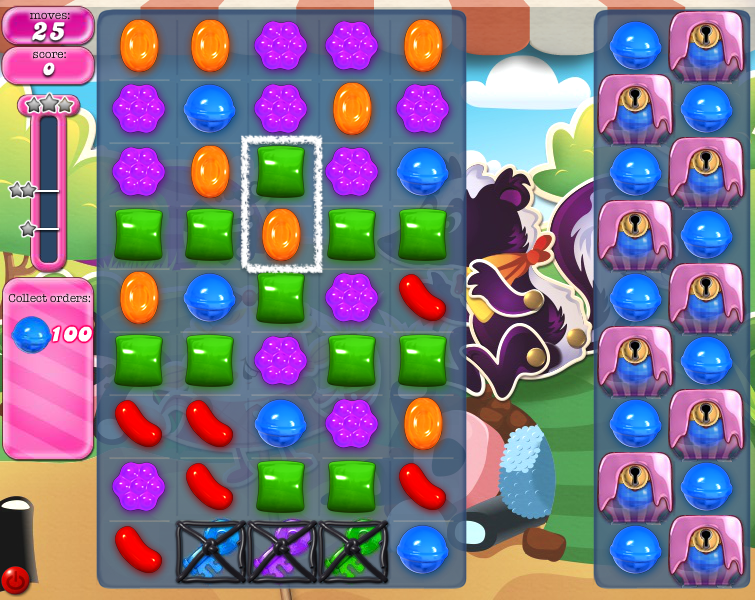
\includegraphics[width=0.4\textwidth]{masters-thesis-master/masters-thesis/contents/02_background/candy_images/Level_1365_Reality.png}
    \label{fig:candy:a}
    }
  \subfloat[]{
    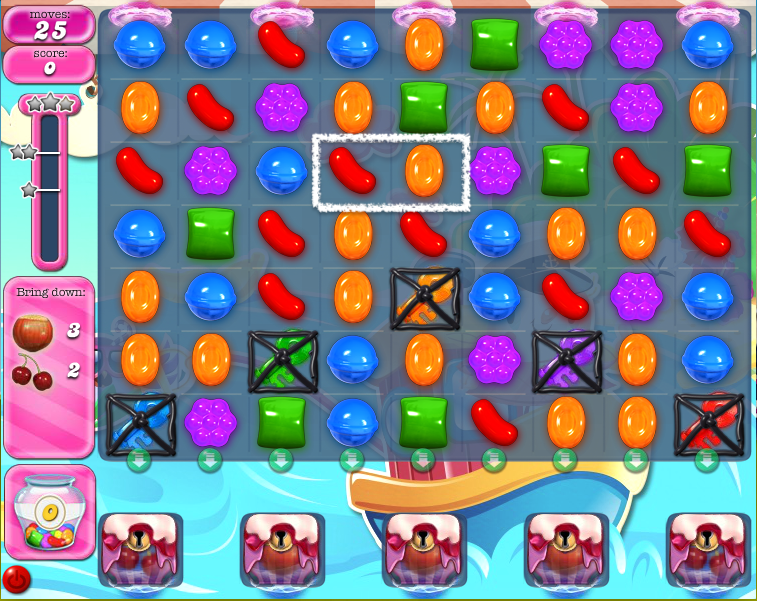
\includegraphics[width=0.4\textwidth]{masters-thesis-master/masters-thesis/contents/02_background/candy_images/Level_1161_Reality.png}
    \label{fig:candy:b}
    }
    
  \subfloat[]{
    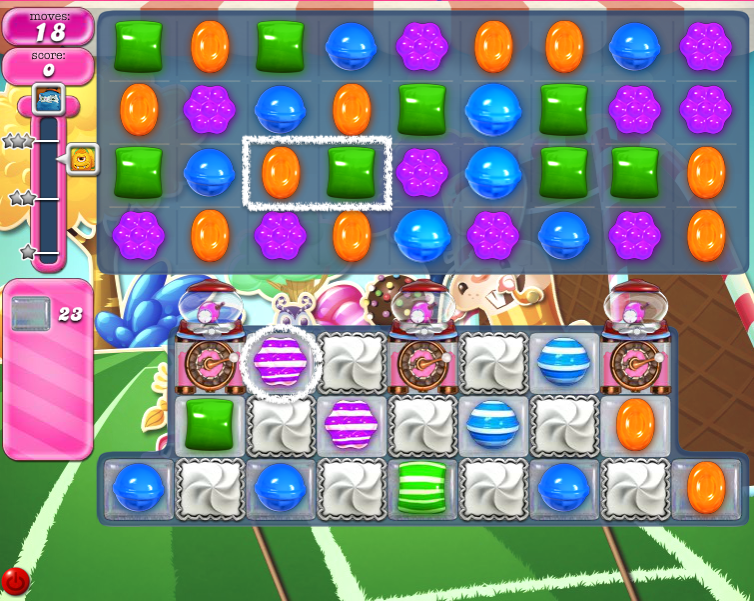
\includegraphics[width=0.4\textwidth]{masters-thesis-master/masters-thesis/contents/02_background/candy_images/Level_1434_Reality.png}
    \label{fig:candy:c}
  }
  \subfloat[]{
    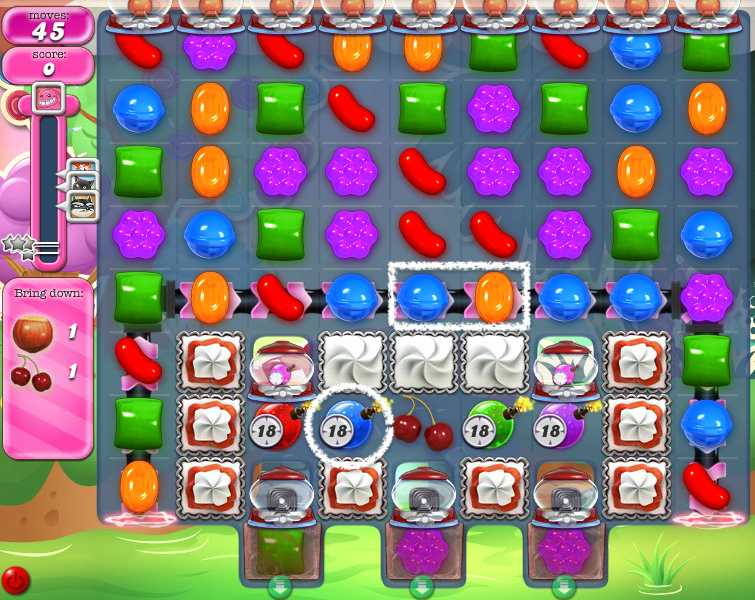
\includegraphics[width=0.4\textwidth]{masters-thesis-master/masters-thesis/contents/02_background/candy_images/Level_963_Reality.png}
    \label{fig:candy:d}
  }
  
    \caption{Examples of legal moves in the game and examples of items. White boxes illustrate examples of possible swaps while white circles illustrate special candies or items.
    }
    \label{fig:candy}
\end{figure}

Figure \ref{fig:candy} shows four different game states and various types of candies and items of four different game levels.  In Figure \ref{fig:candy:a} the white box shows a possible swap that, if executed, creates a special candy called "Colour Bomb" that when switched with a regular candy, it deletes all the candies of that colour from the board. In Figure \ref{fig:candy:b} the white box illustrates a swap that creates a "Striped Candy". When a "Striped Candy" is matched, it deletes all the candies in its row or column. In Figure \ref{fig:candy:c} the white box shows a regular swap while the circle illustrates a "Horizontal Striped Candy". In Figure \ref{fig:candy:d} the white circle shows a "Candy Bomb" with a timer of 18 available moves before it explodes and the player loses the game. Also, the white box shows a regular swap on a "Conveyor Belt" that is an item that moves the candies on it by one position in the direction of the belt every turn. Moreover, the examples in Figures \ref{fig:candy} contain a lot of others special items, each one with its own characteristics and effects. The images in Figure \ref{fig:candy} show different level objectives. The level in Figure \ref{fig:candy:a} is a \textit{candy order level}, the level in Figure \ref{fig:candy:c} is a \textit{jelly level} while levels in Figure \ref{fig:candy:b} and \ref{fig:candy:d} are examples of \textit{ingredients levels}. This illustrates the diversity between the levels in the game.

The game allows players to use boosters (sometimes known as power-up). A booster is an item that can be used to facilitate the gameplay and solving a level more easily. In \textit{Candy Crush Saga} there are 15 different boosters each one with different properties. They can be grouped into three main categories:
\begin{enumerate}
    \item \textbf{Pre-level boosters.} Activated before the game starts.
    \item \textbf{In-level boosters.} Activated during the gameplay if the conditions of the game board create any effect when the booster is used. As an example, a player cannot use a "Bomb Cooler" booster if there are no "Bombs" on the game board.
    \item \textbf{Consolation boosters.} Activated at the end of the attempt to prevent failure and retrying.
\end{enumerate}
Each booster has a number of charges. Every time a player uses a booster, one charge is consumed. Some boosters can be used only in specific type of levels. In Appendix \ref{boosters} a full description of all the boosters with their effects and usage conditions.


\subsection{Gameplay Metrics}
In the last years, game metrics have become popular in the game industry as a source of valuable information about game design. Game metrics are the result of the interaction between the players and the game. Compared to user feedback or surveys, game metrics have the advantage to be objective, not biased by player emotions and they are easier to gather on a large scale. Since our goal is to estimate level difficulty, we use the \acs{sr} on a specific level as a measure of the perceived difficulty. The success rate $sr_{i,k}$ on a level $i$ perceived by a group of players $k$ is defined as follow:
\begin{equation}
 sr_{i,k}= \frac{s_{i,k}}{a_{i,k}} \text{,}
\end{equation}
 \label{eq:sucess_rate}
where $s_{i,k}$ is the sum of the number of successes on level $i$ of each player in group $k$ and $a_{i,k}$ is the sum of the number of attempts on level $i$ of each player in the considered group $k$. The reason why we use the \acs{sr} as a measure of the perceived difficulty is because we believe that if a player needs to try a level many times before solving it, and thus the \acs{sr} is low, he perceives the level as a difficult one, while on the contrary, if a player solves a level in few attempts, he perceives the level as an easy one and the \acs{sr} is high. Another reason why we use the \acs{sr} is to allow a comparison with the state-of-the-art approach. However, since the baseline does not consider different groups of players, we furthermore use a combination of the SR of all the $k$ groups to estimate $sr_{i}$ that is the overall difficulty perceived by all the players on level $i$.

\subsection{Related Work}
Until \textcite{silver_mastering_2016} published their work in 2016, presenting the Google DeepMind’s \textit{AlphaGo} system, most of the research in the game of \textit{Go} was focused on \acs{RL} to teach computer playing the game. The state-of-the-art were \acs{MCTS} programs that simulates thousands of self-play games to estimate the optimal policy. \textcite{silver_mastering_2016} demonstrated how deep neural networks trained on human expert player data can effectively estimate the "value network" used to evaluate board positions and approximate the "policy network" used to select moves in the game of \textit{Go}. The two networks were trained by a combination of reinforcement learning and supervised learning using human expert data. Their research was based on prior work on predicting expert moves in the game of  \textit{Go} using supervised learning techniques \cite{sutskever_mimicking_2008, stern_bayesian_2006, maddison_move_2014}. Their solution is the first computer \textit{Go} program that beat a human professional \textit{Go} player without handicaps. In 2015, \textit{AlphaGo} defeated Fan Hui, a three times European \textit{Go} champion, in all of the 5 matches disputed. In 2016, it beat Lee Sedol, a 9-dan professional player considered one of the best players at \textit{Go}, in a five-game match. 

Similarly to what Silver \textit{et al.} did with \textit{AlphaGo}, \textcite{hlynur_predicting_2017} illustrated how \acs{CNN} can be designed to predict expert moves for the \textit{Othello} game, exceeding the previous state-of-the-art by 5.3\%. He used a \acs{DCNN} trained with handcrafted features and the raw board state as input, showing that removing the handcrafted features decreases the accuracy by only 0.9\% but at the same time allows for a much faster computation. \textcite{chen_game_2017} demonstrated that \acs{CNN} can provide similar performance while requiring fewer resources and training time compared to more complex methods such as deep Q-learning in challenging policy estimation task. More recently, the new Google \textit{AlphaGo Zero} program \cite{silver_mastering_2017} trained solely by self-play reinforcement learning achieved super-human performances, winning 100-0 against the previously published \textit{AlphaGo} system. However, a perfect-play agent that always plays the optimal move and leads to the best possible outcome is out of the scope of this thesis. We aim to model human players and even the best player does not always select the optimal action due to the difficulty of identifing and evaluating each possible move in the \textit{Candy Crush Saga} game. For this reason, it is important that the \acs{AI} agent plays in a human-like manner, making the same sort of errors and therefore using a similar strategy to human players. 

The game of \textit{Go} has several similarities with the game used in our research. First, the grid shape topology of the board and the discrete game action space that make \acs{CNN} a valid approach to simulate gameplay. Second, the vast search space that makes computationally hard to evaluate each possible state-action pair in the game. Third, the observability, since both games have perfect information. Fourth, the time granularity, since both are turn based games and finally, the Markov property, that practically holds for both the games. \textit{Candy Crush Saga} can be considered, for practical purposes, to have the Markov property, even if there are few special cases where specific game items violate this assumption. There is a special candy called "Chameleon candy" that alternates between two colors every turn. However, since this type of candy is really rare in the game, we will treat the game as a Markov process. Even if there are some differences, like the fact that \textit{Go} is a two player zero-sum adversarial game while \textit{Candy Crush Saga} is a single player game or that \textit{Go} is deterministic while \textit{Candy Crush Saga} it is not, we rely on the results of previous work in the game of \textit{Go} to guide our research. Finally, in the last three years, some related work on the \textit{Candy Crush Saga} game has been done. As mentioned in Section \ref{Automatic Playtesting Related Work},  \textcite{poromaa_crushing_2017} used a \acs{MCTS} approach while \textcite{eisen_simulating_2017} and \textcite{purmonen_predicting_2017} used a \acs{CNN}-based approach to simulate gameplay, similarly to what have been done in the \textit{AlphaGo} system.

\section{Theory}

\subsection{Linear Regression}

Linear regression is one of the simplest approach for regression analysis. It models a linear relationship between a dependent variable and one or more independent variables, also called explanatory variables or predictors. Linear regression is largely applied in biological, behavioural and social sciences as well as finance and economics to describe the relationships between different variables. Linear regression models are used both for prediction and for quantifying the relationship between response and explanatory variables. When it is used for prediction, as in this thesis, a linear regression model is obtained by fitting the observed training data. Then, if new values of the explanatory variables are collected, the model is used to predict the response variables.

Given a data set $\{y_{i}, x_{i1}, \dots, x_{id}\}^{n}_{i=1}$ where $n$ is the number of examples in the data, $y$ is the response variable and $\mathbf{x}$ is the d-vector that describes the explanatory variables, the linear relationship is modeled as:
\begin{equation}
    y_i = \beta_01 + \beta_1x_{i1} + \dots + \beta_dx_{id} + \epsilon_i \text{,}  \qquad i=1,\dots,n \text{,}
\end{equation}
where $\epsilon_i$ is the error term that adds noise to the linear relationship. If written in matrix form the linear equations can be expressed as:
\begin{equation}
    \mathbf{y} = {\mathbf{X}\bm{\beta}} + \bm{\epsilon} \text{,}  
\end{equation}
where 
\begin{equation}
    \mathbf{y} = \begin{pmatrix} y_1 \\ y_2 \\ \vdots \\ y_n\end{pmatrix}\text{,} \quad
    \mathbf{X} = \begin{bmatrix} 1 & x_{11} & \dots & x_{1d}  \\ 
                                 1 & x_{21} & \dots & x_{2d}  \\   
                                 \vdots & \vdots & \ddots & \vdots \\
                                 1 & x_{n1} & \dots & x_{nd} \\
                                 \end{bmatrix}\text{,} \quad
    \bm{\beta} = \begin{pmatrix} \beta_0 \\ \beta_1 \\ \vdots \\ \beta_d\end{pmatrix}\text{,} \quad
    \bm{\epsilon} = \begin{pmatrix} \epsilon_1 \\ \epsilon_2 \\ \vdots \\ \epsilon_n\end{pmatrix}\text{.}
\end{equation}
Several procedures to estimate the parameters $\bm{\beta}$ have been proposed. One of the most popular is \acf{OLS} since it leads to a closed-form solution. It computes the estimated values $\hat{\bm{\beta}}$ by minimizing the sum of squared residuals. The estimates are computed as: 
\begin{equation}
    \hat{\bm{\beta}} = {(\mathbf{X}^\top\mathbf{X})^{-1}\mathbf{X}^\top\mathbf{y}}   
\end{equation}
If the errors have finite variance and are uncorrelated with the predictors then the estimator is consistent and unbiased.
\begin{equation}
    \mathbb{E}[\mathbf{x}_i \epsilon_i] = 0   
\end{equation}
\acs{OLS} method computes the best fitting line for the observed data. Furthermore, once a regression model has been fit, an examination of the deviations of the observed values from the fitted line (residuals), allows to investigate the validity of the obtained linear model. For more information regarding linear regression analysis we refer to \cite{montgomery_introduction_2012}.


\subsection{Convolutional Neural Networks}
A \acl{CNN} is a specific type of feed-forward artificial neural network that uses a shared-weights architecture and has the translation invariance property. It is mainly used for processing data with a grid-like topology, e.g. time series or images. \acsp{CNN} were inspired by the animal visual cortex where neurons are activated by stimuli from a restricted region of the visual field. A \acs{CNN} consists of an input layer, an output layer and a variable number of hidden layers. Layers can be repeated many times and the output of one layer becomes the input of the next one. An example of a \acs{CNN} architecture is illustrated in Figure \ref{fig:network_architecture_example}.

A key characteristics of \acsp{CNN} is that they have sparse connectivity, meaning that when a convolution operation is performed, the output is determined only by a subset of the input (called receptive field) that depends on the size of the filters. However, in a deep \acs{CNN}, deeper layers may have indirect connections with larger subset of the input. This enable the network to learn complex functions combining simple building blocks. Each hidden layer typically consists of one of the following three types: a convolutional layer, a pooling layer or a fully connected layer. \\ \\

\begin{figure}[ht]
    \centering
    
	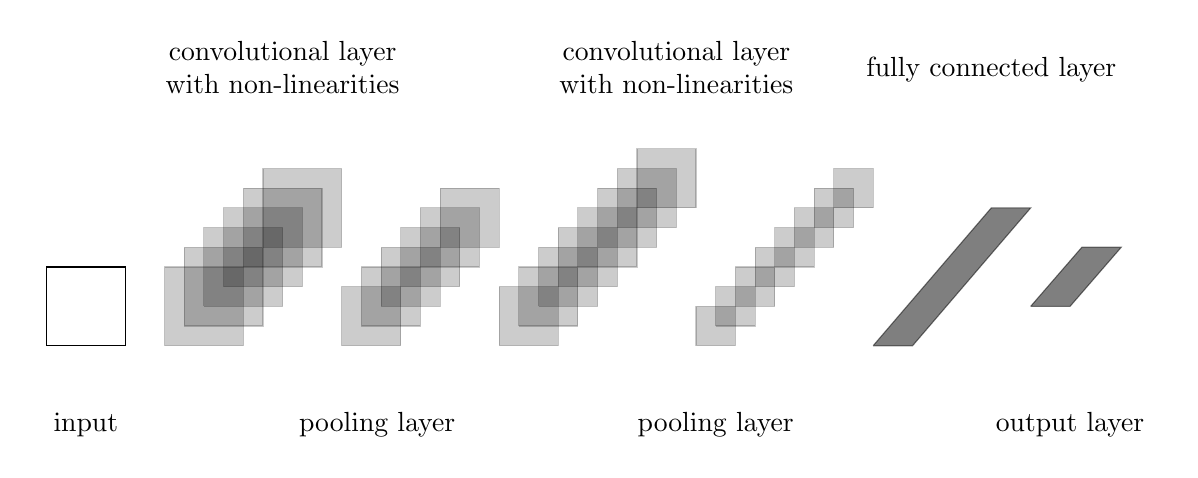
\begin{tikzpicture}
		\node at (0.5,-1){\begin{tabular}{c}input\end{tabular}};
		
		\draw (0,0) -- (1,0) -- (1,1) -- (0,1) -- (0,0);
		
		\node at (3,3.5){\begin{tabular}{c}   convolutional layer\\   with non-linearities \end{tabular}};
		
		\draw[fill=black,opacity=0.2,draw=black] (2.75,1.25) -- (3.75,1.25) -- (3.75,2.25) -- (2.75,2.25) -- (2.75,1.25);
		\draw[fill=black,opacity=0.2,draw=black] (2.5,1) -- (3.5,1) -- (3.5,2) -- (2.5,2) -- (2.5,1);
		\draw[fill=black,opacity=0.2,draw=black] (2.25,0.75) -- (3.25,0.75) -- (3.25,1.75) -- (2.25,1.75) -- (2.25,0.75);
		\draw[fill=black,opacity=0.2,draw=black] (2,0.5) -- (3,0.5) -- (3,1.5) -- (2,1.5) -- (2,0.5);
		\draw[fill=black,opacity=0.2,draw=black] (1.75,0.25) -- (2.75,0.25) -- (2.75,1.25) -- (1.75,1.25) -- (1.75,0.25);
		\draw[fill=black,opacity=0.2,draw=black] (1.5,0) -- (2.5,0) -- (2.5,1) -- (1.5,1) -- (1.5,0);
		
		\node at (4.2,-1){\begin{tabular}{c}pooling layer \end{tabular}};
		
		\draw[fill=black,opacity=0.2,draw=black] (5,1.25) -- (5.75,1.25) -- (5.75,2) -- (5,2) -- (5,1.25);
		\draw[fill=black,opacity=0.2,draw=black] (4.75,1) -- (5.5,1) -- (5.5,1.75) -- (4.75,1.75) -- (4.75,1);
		\draw[fill=black,opacity=0.2,draw=black] (4.5,0.75) -- (5.25,0.75) -- (5.25,1.5) -- (4.5,1.5) -- (4.5,0.75);
		\draw[fill=black,opacity=0.2,draw=black] (4.25,0.5) -- (5,0.5) -- (5,1.25) -- (4.25,1.25) -- (4.25,0.5);
		\draw[fill=black,opacity=0.2,draw=black] (4,0.25) -- (4.75,0.25) -- (4.75,1) -- (4,1) -- (4,0.25);
		\draw[fill=black,opacity=0.2,draw=black] (3.75,0) -- (4.5,0) -- (4.5,0.75) -- (3.75,0.75) -- (3.75,0);
		
		\node at (8,3.5){\begin{tabular}{c}convolutional layer\\with non-linearities \end{tabular}};
		
		\draw[fill=black,opacity=0.2,draw=black] (7.5,1.75) -- (8.25,1.75) -- (8.25,2.5) -- (7.5,2.5) -- (7.5,1.75);
		\draw[fill=black,opacity=0.2,draw=black] (7.25,1.5) -- (8,1.5) -- (8,2.25) -- (7.25,2.25) -- (7.25,1.5);
		\draw[fill=black,opacity=0.2,draw=black] (7,1.25) -- (7.75,1.25) -- (7.75,2) -- (7,2) -- (7,1.25);
		\draw[fill=black,opacity=0.2,draw=black] (6.75,1) -- (7.5,1) -- (7.5,1.75) -- (6.75,1.75) -- (6.75,1);
		\draw[fill=black,opacity=0.2,draw=black] (6.5,0.75) -- (7.25,0.75) -- (7.25,1.5) -- (6.5,1.5) -- (6.5,0.75);
		\draw[fill=black,opacity=0.2,draw=black] (6.25,0.5) -- (7,0.5) -- (7,1.25) -- (6.25,1.25) -- (6.25,0.5);
		\draw[fill=black,opacity=0.2,draw=black] (6,0.25) -- (6.75,0.25) -- (6.75,1) -- (6,1) -- (6,0.25);
		\draw[fill=black,opacity=0.2,draw=black] (5.75,0) -- (6.5,0) -- (6.5,0.75) -- (5.75,0.75) -- (5.75,0);
		
		\node at (8.5,-1){\begin{tabular}{c}pooling layer \end{tabular}};
		
		\draw[fill=black,opacity=0.2,draw=black] (10,1.75) -- (10.5,1.75) -- (10.5,2.25) -- (10,2.25) -- (10,1.75);
		\draw[fill=black,opacity=0.2,draw=black] (9.75,1.5) -- (10.25,1.5) -- (10.25,2) -- (9.75,2) -- (9.75,1.5);
		\draw[fill=black,opacity=0.2,draw=black] (9.5,1.25) -- (10,1.25) -- (10,1.75) -- (9.5,1.75) -- (9.5,1.25);
		\draw[fill=black,opacity=0.2,draw=black] (9.25,1) -- (9.75,1) -- (9.75,1.5) -- (9.25,1.5) -- (9.25,1);
		\draw[fill=black,opacity=0.2,draw=black] (9,0.75) -- (9.5,0.75) -- (9.5,1.25) -- (9,1.25) -- (9,0.75);
		\draw[fill=black,opacity=0.2,draw=black] (8.75,0.5) -- (9.25,0.5) -- (9.25,1) -- (8.75,1) -- (8.75,0.5);
		\draw[fill=black,opacity=0.2,draw=black] (8.5,0.25) -- (9,0.25) -- (9,0.75) -- (8.5,0.75) -- (8.5,0.25);
		\draw[fill=black,opacity=0.2,draw=black] (8.25,0) -- (8.75,0) -- (8.75,0.5) -- (8.25,0.5) -- (8.25,0);
		
		\node at (12,3.5){\begin{tabular}{c}fully connected layer \end{tabular}};
		
		\draw[fill=black,draw=black,opacity=0.5] (10.5,0) -- (11,0) -- (12.5,1.75) -- (12,1.75) -- (10.5,0);
		
		\node at (13,-1){\begin{tabular}{c}output layer \end{tabular}};
		
		\draw[fill=black,draw=black,opacity=0.5] (12.5,0.5) -- (13,0.5) -- (13.65,1.25) -- (13.15,1.25) -- (12.5,0.5);
	\end{tikzpicture}
	\caption[Architecture of a traditional convolutional neural network.]{Example of a CNN architecture. As first introduced by LeCun et al. in 1989, this network alternates between convolutional layers with hyperbolic tangent activation functions to introduce non-linearities and pooling layers. In this representation, the convolutional layers include the activation functions. The grey squares represent the activation maps. The last two layers are fully connected layers. Usually, the output layer uses a softmax activation function. Image generated with code adapted from \cite{stutz_latex-resources:_2018}. }


%    \input{contents/03_method/i00_network_architecture_horizontal}
    \label{fig:network_architecture_example}
\end{figure}
\noindent
\textbf{Convolutional layer:} It applies a convolutional operation to the input and it drastically reduces the number of free parameters allowing to operate with inputs that have high dimensionality like images. Instead of having a connection from each input to each output, as in a fully connected feed-forward neural network, it uses filters (typically of a small size, e.g. 3x3) that are shared between inputs. In this way, each parameter of the filter is used in every position of the input, with various design choices for managing the boundaries. The filters are moved step by step over the input and at each step, the dot product between the filter and the input is computed. The number of units by which the filters shift over the input is the filter stride. On top of that is typically added a non-linear activation function. Each convolutional layer uses one or more filters and each of them, moving over the input, generates an activation map. Finally, all the generated activation maps are stacked together and they constitute the input of the next layer. As a result, the network learns filters that are activated when they detect specific features in the input. Sometimes batch normalization is added at the beginning of the convolutional layer to speed up training and to reduce overfitting. \\ \\
\textbf{Pooling layer:} It reduces the size of each activation map combining multiple outputs of a convolutional layer into a single value. In practice, many types of pooling layers exist and as an example the \textit{max pooling layer} combines multiple output of the previous layer retaining only the maximum value. The idea is to generate smaller representations maintaining only the relevant information introducing invariance to small shifts or distortions. Furthermore, the pooling layer progressively decreases the size of the representation, reducing the number of parameters and the amount of computation required by the network.\\ \\
\textbf{Fully connected layer:} A fully connected layer connects every neuron in the input to every neuron in the output. This type of layer is usually added at the end of the network to feed a \textit{softmax} function and generate a distribution over the output classes. \textcite{lin_network_2013} proposed another strategy called \acf{GAP} to replace the fully connected layers. When using \acs{GAP}, the last convolutional layer has to generate one feature map for each target class. Then, instead of having a fully connected layer, the average of each feature map is computed and the output is fed into a \textit{softmax} function. The advantage of this approach is that since there are no parameters to optimize in the \acs{GAP} layer, overfitting is avoided at this layer. Finally, since from each map only the average value is retained the network is more robust to input spatial translations.\\ \\
The idea of \acs{CNN} \cite{lecun_backpropagation_1989, fukushima_neocognitron:_1980} dates back to the 80s. One of the first applications was to recognize hand-written digits on checks or mails but due to slow computational resources and limited amount of labeled data the research on \acsp{CNN} progressed slowly until 2012. In that year, \textcite{krizhevsky_imagenet_2012} famously developed a network called "AlexNet" and they won, by a large margin, the \acf{ILSVRC} \cite{russakovsky_imagenet_2015}. After this successful result, many variants of \acsp{CNN} have been proposed and new applications have been found. At the time of writing, examples of the most popular and prominent architectures are the inception network and the residual network. The inception network architecture \cite{szegedy_rethinking_2016} was introduced by Google and mainly consists of parallel 1x1, 3x3 and 5x5 convolutional filters combined into several modules. This architecture is able to reduce the number of features, and so the performed operations, compared to the ones of "AlexNet", leading to a very efficient architecture. The main idea of the residual network \cite{he_deep_2016} is to add skip connections allowing the output of a convolutional layer to bypass the next two layers. This approach helps the learning of deep \acsp{CNN} with many layers by better gradient backpropagation. For a deeper understanding about \aclp{NN} and their applications we refer to \cite{goodfellow_deep_2016}.

\subsection{Clustering}

Clustering is an exploratory data mining process that consists of grouping together objects such that elements in the same group (called cluster) are more similar compared to elements in different groups. The term "clustering" refers to the general task and many algorithms to perform it have been proposed. In this thesis we use hierarchical clustering and k-means.

\subsubsection*{Hierarchical clustering}

The algorithm iteratively connects elements to form clusters based on distances between elements. Two main hierarchical clustering approaches exist: the top-down approach starts considering all the elements as a single cluster and iteratively splits them into smaller ones, while the bottom-up approach starts considering all the elements as single clusters and iteratively merges them. Different distance functions can be used, e.g. euclidean distance, hamming distance, cosine distance. Also, the user needs to chose the linkage function, since a cluster consists of multiple data point, the algorithm needs a criterion to select which element to use when computing the distance function. Popular linkage functions are the \textit{single-linkage} function, the \textit{complete-linkage} function and the \textit{average-linkage} function. The \textit{single-linkage} function, considers the minimum of the element distances. As a consequence, the distance $D(X,Y)$ between two clusters $X$ and $Y$ is described by: 
\begin{equation}
 D(X,Y)= \min_{x\in X,y\in Y} d(x,y)  \text{,}
\end{equation}
 \label{eq:single_linkage}
 where $d(x,y)$ denotes the distance between two elements $x$ and $y$. The
\textit{complete-linkage} function considers the maximum of the element distances and it is described by:
\begin{equation}
 D(X,Y)=\max_{x\in X,y\in Y} d(x,y)  \text{,}
\end{equation}
 \label{eq:complete_linkage}
 instead, the \textit{average-linkage} function, also known as \textit{\acl{UPGMA}} (\acs{UPGMA}), considers the average of the element distances and it is described by:
 \begin{equation}
 D(X,Y)=\sum_{x\in X,y\in Y} \frac{d(x,y)}{|X|\cdot|Y|}  \text{,}
\end{equation}
 \label{eq:average_linkage}
 where $|X|$ and $|Y|$ are the cardinalities of clusters $X$ and $Y$ respectively.
Finally, since the general complexity of hierarchical clustering is $\mathcal{O}(n^3)$ this algorithm performs well only for small data sets. However, it does not produce a single partitioning but an extensive hierarchy of merged clusters that can be visualized with a two dimensional diagram known as dendogram \cite{everitt_hierarchical_2011}. Example of a dendogram is illustrated in Figure \ref{fig:dendogram_example}. We can observe how starting with six separate data points the algorithm iteratively merges them until a single cluster containing all the points is obtained.
\begin{figure}[h]
    \centering
    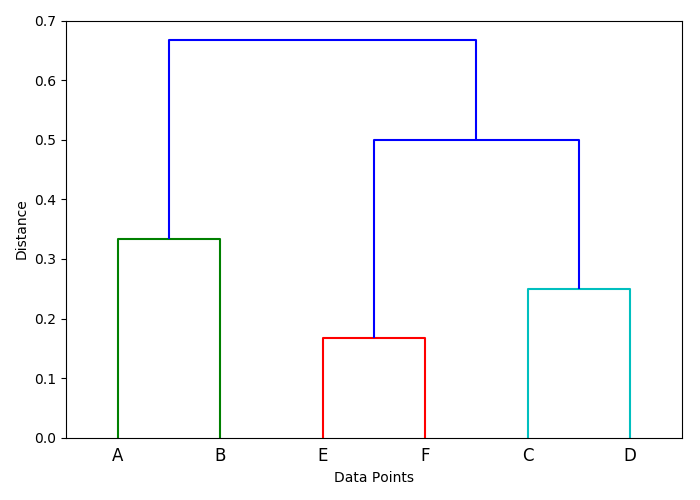
\includegraphics[width=0.6\textwidth]{masters-thesis-master/masters-thesis/contents/02_background/dendogram_example.png}
    \caption{Example of a dendogram. On the x-axis the data points to be clustered, on the y-axis the distance measure. The distance between merged clusters is monotone increasing with the level of the merger. The height of each merge is proportional to the dissimilarity between the data points in each merged cluster. Using a bottom-up approach, the first generated cluster is \{E,F\}, then the second generated cluster is \{C,D\}, the third is \{A,B\} and finally, the last two clusters: \{E,F,C,D\} and the cluster with all the data points \{A,B,E,F,C,D\}.}
    \label{fig:dendogram_example}
\end{figure}

\subsubsection*{K-means}
The algorithm was introduced in 1976 by Stuart Lloyd \cite{lloyd_least_1982}, which is why it is also referred as Lloyd's algorithm, however it was not published outside the Bell labs until 1982 and the term "k-means" was introduced in the same year by James MacQueen. The algorithm aims to partition $n$ observations into $k$  $(\leq n)$ clusters in which each observation belongs to the cluster with the nearest mean. 

\noindent
More formally, given a set of observations $(x_1, x_2, \dots, x_n)$, where each observation is a d-dimensional array, k-means partitions the $n$ observations into $k$ sets $S = {S_1, S_2, \dots, S_k}$ trying to minimize the \acf{WCSS} distances:
\begin{equation}
    \arg\min_{S} \sum_{i=1}^{k} \sum_{x \in S_i} \lVert x - \mu_i \rVert^2 \text{,}
\end{equation}
where $\mu_i$ is the mean of the points in $S_i$.
The most common version of the algorithm uses iterative refinement to assign each observation to a cluster. The number of clusters $k$ is an input parameter of the algorithm and its choice significantly impacts the quality of the output.
The algorithm, starting with a set of k-means, alternates between two steps until convergence:
\begin{enumerate}
    \item Assignment step: assign each observation to the nearest cluster,
    \item Update step: compute the new means of each cluster, called centroids.
\end{enumerate}
The algorithm converges when no observation changes cluster during the assignment step, however it does not guarantee to find the optimal solution.
A common approach to select the parameter $k$ is the elbow criterion \cite{wierzchon_cluster_2018}. The main idea is to run the algorithm for a range of values of $k$ and computing the \acf{SSE} for each value. Plotting the SSE against the number of clusters $k$, we can chose $k$ by looking at the "elbow" of the line. The idea is to select a small value of $k$ that still has a low SSE. Sometimes this value cannot be unambiguously identified. Regarding the initialization of the centroids, many variants have been proposed and a common approach is to randomly initialize them. For more details about k-means we refer to \cite{wu_advances_2012}.







